\documentclass[sigconf,nonacm,article]{acmart}
\usepackage{array}

\setcopyright{none}

\begin{document}
\title{PDU Protocol: A Peer-to-Peer Social Netwrok Service}
\author{Peng Liu}
\email{liupeng@pdu.pub}

\begin{abstract}
   A fully peer-to-peer (P2P) social networking system should enable participants to freely publish and efficiently access information without relying on any third-party services. However, if the system does not employ centralized verification methods, such as phone numbers, allowing the cost-free creation of new accounts, it becomes susceptible to Sybil attacks. This vulnerability undermines the system’s reward and punishment mechanisms, inundates genuine content with spam, and renders the system unusable. This paper proposes a solution for constructing a P2P social network without relying on any third-party user authentication services. The scheme establishes a trusted publisher identity through a sequence of messages signed by the same private key. Interactions such as reposts, comments, and likes create associations between publishers. Based on these associations, participants can form a custom set of visible publisher identities. Within this relatively stable scope, an identity-based reward and punishment mechanism can be employed to effectively filter information.
\end{abstract}

\maketitle
\pagestyle{plain} % add page numbers, remove title/authors in the page header

\section{Introduction}\label{sec:introduction}

The dissemination and interaction of information on today's internet primarily rely on centralized platforms such as Facebook, Twitter/X, and WeChat. These platforms allow users to conveniently publish information and establish connections, employing algorithms to detect and filter spam to ensure user experience. However, as these platforms have evolved, the issues associated with centralized social services have become increasingly apparent. Third-party services may misuse user information or lead to data breaches. They might exploit their vast user base to lock in users and maintain their monopoly. Additionally, centralized services are susceptible to government regulation and censorship since they are controllable entities.

Despite these issues, we are compelled to continue using these platforms. For most people, switching platforms does not result in data loss but leads to the loss of user relationships accumulated on the platform, thereby reducing their influence. This is a significant reason why users are largely locked into these platforms.

There are some decentralized social platforms, such as Mastodon~\cite{Trust} and Diaspora. Mastodon's federated architecture and Diaspora's distributed architecture share some commonalities: both consist of multiple interconnected servers, and users can maintain their own association relationships. However, user registration and content management still rely on the administrators of each server. This governance structure can be seen as a combination of multiple small centralized platforms, each with its own rules and management methods, and users still cannot fundamentally avoid the issues encountered in centralized platforms.

There are also some blockchain-based decentralized social platforms such as Steemit and Minds. They require a certain number of tokens as the cost to create or activate accounts and also use tokens as incentives for social behavior. While this method appears to impose a cost on account creation, it fundamentally differs from the costs associated with centralized platforms. When the benefits a single account can bring exceed the creation cost, this restrictive method becomes entirely ineffective.

This paper proposes a new peer-to-peer (P2P) social network system. This system does not rely on any third-party services. Any sequence of messages signed with the same private key and having a total order is recognized by the system as a legitimate publisher identity. Through interactions between messages, public associations can be formed between publisher identities. Any user can maintain a visible set of publisher identities according to custom rules based on these associations and effectively filter information within this scope using the publisher's identity as a marker.

\section{Messages}\label{sec:messages}

Messages are defined as the fundamental data structure within the system and constitute the only type of information transmitted in the peer-to-peer network. Other data types in the system, such as publisher identities, are derived from this publicly available data and are autonomously generated by individual nodes.

\begin{figure}
   \centering
   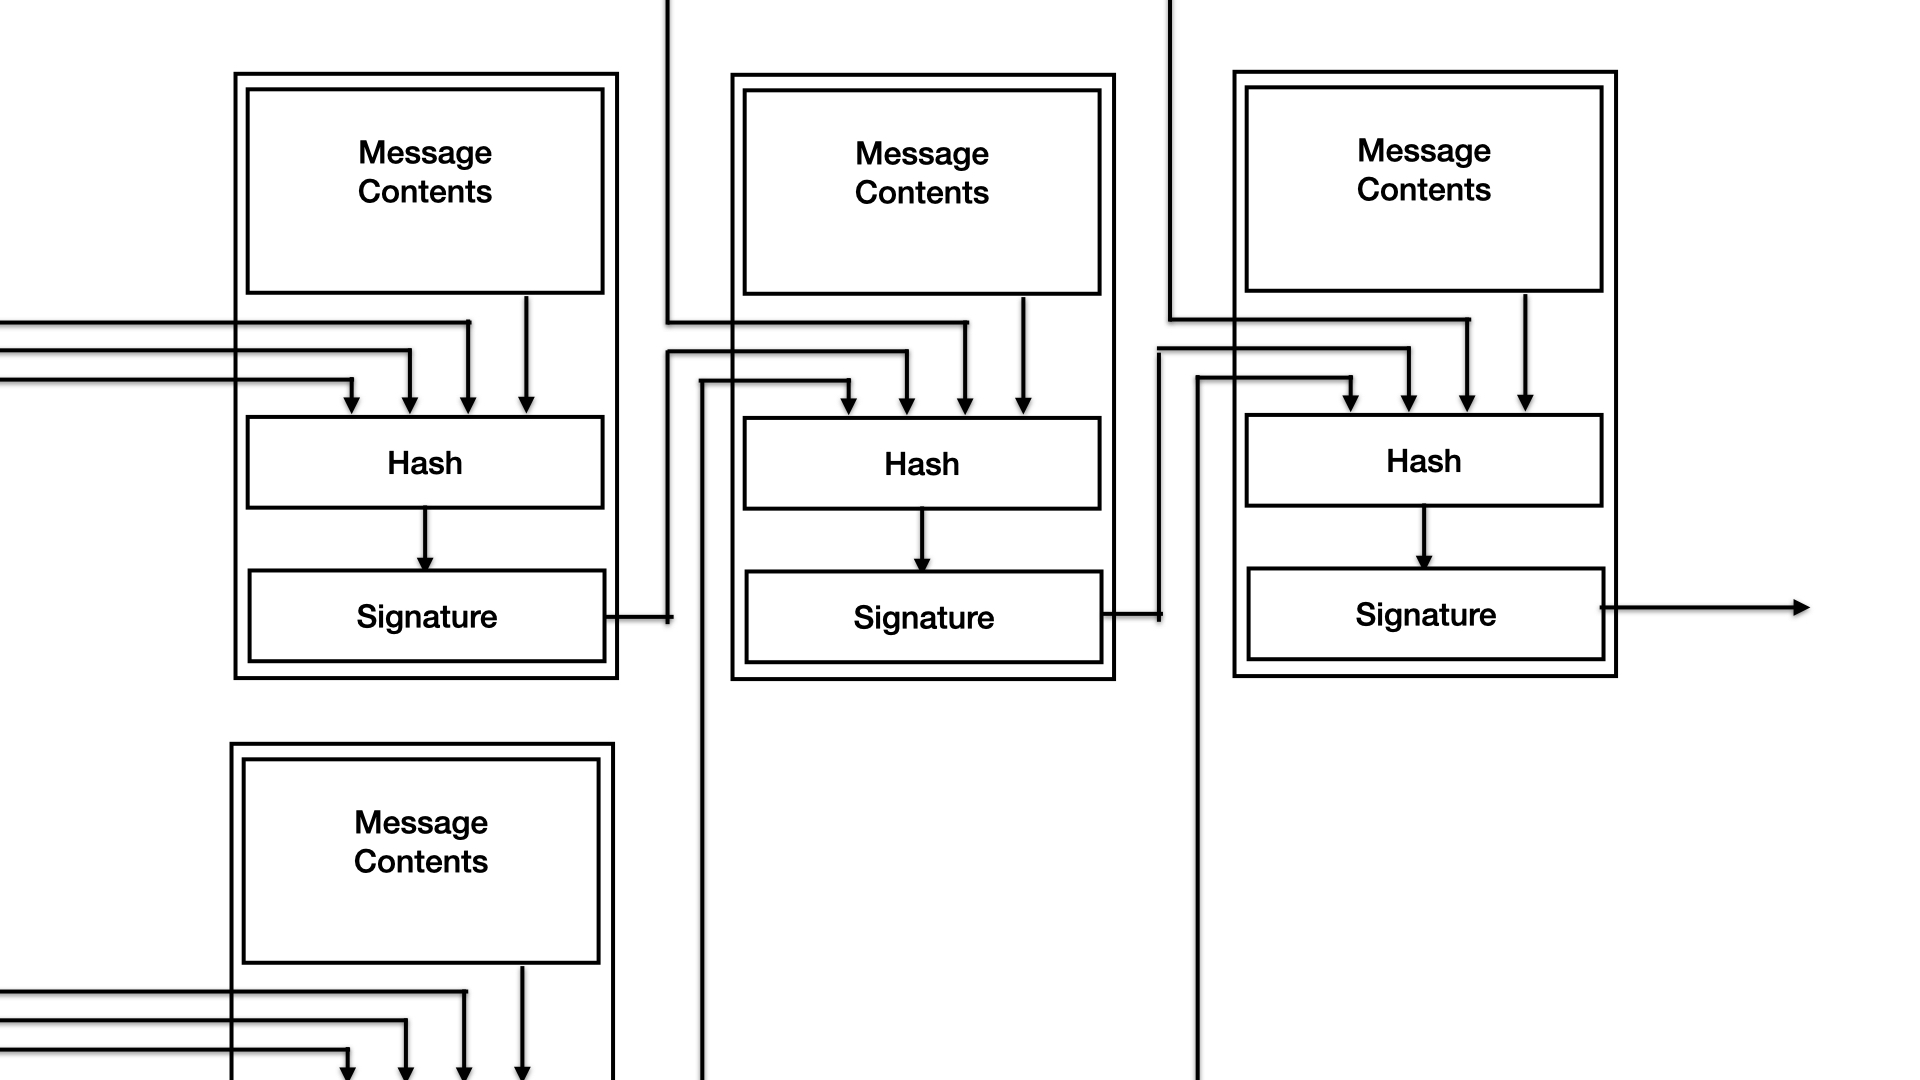
\includegraphics[width=1\linewidth]{MsgLink.jpeg}
   \caption{Structure of messages and their interconnections in the network. }
   \label{fig:message}
\end{figure}

Each message consists of three parts: the message content, the reference list, and the signature (see Figure~\ref{fig:message}). The message content forms the main body of the message, divided into content information and interaction types. The former includes text, images, etc., while the latter encompasses common social network interactions such as posting, replying, referencing, and liking. The reference list can contain the signatures of multiple messages to indicate the temporal relationship between the current message and the referenced messages. When the message content involves interaction types such as replying or referencing, the signatures of the related messages should be included in the reference list. To provide more precise temporal verification, it is recommended to include the signature of at least one recent message in the reference list. Finally, the message content and reference list are combined to compute a hash value, which is then signed using the current publisher's private key to confirm the publisher's identity and ensure data integrity.

Although each message has explicit content, it is often impossible to determine whether a message is spam based on the message alone. For instance, messages like "I recommend trying Restaurant A on M Street" or "I advise staying away from Restaurant B on N Street" may seem harmless individually. However, if thousands of similar messages appear in a short period, they would be considered spam. In centralized platforms, this situation is addressed by the platform's filtering mechanisms, which restrict or block the accounts responsible for such posts to prevent legitimate content from being overwhelmed.

Therefore, we need a method to understand the entirety of the information published by an account when necessary and ensure that its published content has not been tampered with. This helps in evaluating the publisher to determine whether their content is normal and whether the publisher should be blocked to reduce spam content. Additionally, we need an account filtering mechanism to prevent the rapid proliferation of new accounts, ensuring that spam publishers cannot continuously repeat the same behavior by frequently changing private keys after being blocked.


\section{Publisher}\label{sec:publisher}

To accurately evaluate an account, we must ensure that the content published by the account has not been tampered with and can be detected if the publisher deletes previously published messages. To achieve this in a peer-to-peer distributed system, we require that the content published by each account forms a linked list structure similar to a blockchain. It is stipulated that the reference list of each message must include the signature of the previous message signed by the same private key as the first reference. If the current message is the first message signed by this private key, the first value in the reference list is set to 0 to indicate the starting point.

In a blockchain system, all miners collaborate to generate a single main chain. Forks in the main chain occur due to competition among miners and are not considered errors. Therefore, the system incentivizes miners through mining rewards and achieves consensus through a consensus mechanism. In this system, message signatures are personal actions, and since signatures cannot be forged, any fork in a publisher's message chain is regarded as intentional modification of historical data, which constitutes malicious behavior. If the first signature in the reference list does not point to a message signed by the current private key, it is also considered malicious behavior. However, if the first message in the reference list is not found, the message is temporarily stored, neither trusted nor penalized. It is the responsibility of the information publisher to maintain a complete message chain signed by themselves, to provide verification in case any message is lost in the network.

Another scenario involves a publisher hiding a forked message chain and releasing messages from another fork into the system only after multiple messages from one fork have been accepted. In this case, the messages already accepted by the system are considered established facts. The typical penalty for the publisher upon detecting a conflict is to discard the messages received after the conflict and block all subsequent messages from the publisher. This approach makes fork attacks meaningless to others.

\section{Visible Identity Set}\label{sec:visible-identity-set}

In a publisher identity system based on message chains signed by the same private key, other participants can easily assess the credibility of an identity and whether it publishes spam, thereby deciding to block it. However, if an identity is blocked, malicious actors can change their signing private key at no cost and continue publishing messages, rendering the punishment mechanism ineffective.

Traditional centralized platforms usually require phone number verification or similar methods to link a user's real identity to the creation of a virtual identity. Some decentralized identity systems, like Sovrin and Civic, employ similar methods, which are relatively reasonable but rely on trusted third-party verification. Some blockchain-based social systems impose a token cost for account creation. However, given the varying wealth conditions of users, it is challenging to find a price that can attract users while suppressing the creation of spam accounts.

In a decentralized social network, we need a limited and variable set of publisher identities. This set can vary for each system user, eliminating the need for uniform rules to define the identity set. In a peer-to-peer distributed system, all information is based on public messages. These messages already include interactions such as comments and likes. From any publisher identity's message chain, we can calculate which publishers they have interacted with and generate multiple identity sets based on different interaction behaviors. These sets can be combined through various set operations to yield different results. For identities in the resultant set, we can further search for publishers who have interacted with them, gradually expanding the number of identities in the visible user set.

It is important to note that the visible identity set is not equivalent to followers on traditional centralized platforms but is more akin to all users on a traditional platform. Only the information published by identities within this scope can be seen by the user. This visible user set can be directly expanded by the user or automatically expanded or reduced according to defined rules. For instance, if a user in the set interacts with another user, the passive party’s identity can be added to the visible identity set. Conversely, if an identity is deemed a spammer, the identity that introduced this spammer to the visible identity set can also be blocked.

When establishing the visible identity set, if the user has one or more publisher identities, these identities can serve as the starting point for expanding the visible set. However, these identities have no essential difference from other identities in the expansion process. There is no binding relationship between a publisher identity and the visible user set.

The visible user set can be considered a custom rule by which users gradually compute their visible user range based on public information. In a peer-to-peer distributed system, the system does not guarantee users access to all information. Hence, even when using the same rules, the final visible identity sets may differ.

Due to the existence of the visible user set, malicious publishers can change private keys and publish information under a new identity at no cost. However, the new publisher identity will not easily be accepted by other users, reducing the spread of spam and its impact on system users. Even if an identity does not publish spam, frequent interactions with punished publishers may lead to its removal from the visible user set by users.

\section{Network}\label{sec:network}

A decentralized network comprises numerous nodes, each generating a relatively fixed hash value for identification. Nodes filter received messages based on their customized visible identity sets. There is no binding relationship between the information publisher and the node address, nor are they restricted by the visible identity set. Publishers can interact with any message, regardless of the node or publisher from which the messages originated. Whether a new message is accepted by a node depends solely on whether the message's publisher is within the node's visible identity set, independent of the original message.

When an identity is accepted by only a few nodes in the network, due to the peer-to-peer message transmission method, many nodes that accept the identity may still be unable to receive new messages because of other nodes' filters. In this scenario, the spread of information is limited, and the message's impact might be minimal. However, through interactive messages such as comments, forwards, references, and likes, the message's reach can be indirectly expanded. High-quality messages often manage to extend their influence and reach through these interactions, leading to broader acceptance by more nodes.

This propagation mechanism helps balance and optimize information dissemination. Although some messages may have a limited initial spread, high-quality content can overcome these initial restrictions through various forms of interaction within the network, expanding its reach and eventually disseminating more widely among nodes.

\section{Incentives}\label{sec:incentives}

In a social network, the measure of a publisher's self-interest lies in the extent of their information dissemination. The primary objective of a publisher can be considered to maximize the spread of their information. Therefore, in this peer-to-peer distributed network, incentives for publishers are reflected in aiding the expansion of their information dissemination, while penalties are aimed at reducing it. Unlike decentralized systems represented by blockchains, social networks do not have a system-wide consensus, and thus, there are no unified incentives or penalties for a publisher's identity. Incentive mechanisms are based on the statistical outcomes of all information recipients' behaviors.

When a publisher consistently produces high-quality content, their content is more likely to interact with other publishers. Through these interactive messages, the current publisher's content is more likely to be accepted by nodes that have not yet included the current publisher's identity in their visible identity set. As more nodes accept their identity, the number of nodes that can directly receive their messages increases when they broadcast them. This process allows the content of the current publisher to gain an increasingly wider reach over time.

Conversely, if a publisher consistently posts spam or frequently interacts with spam messages, other publishers will be less inclined to interact with them. Some nodes that have already accepted the current publisher's identity may remove this address from their visible user set. Thus, the behavior and content quality of a publisher directly affect the reach and impact of their information. Here, spam refers not only to messages containing explicit content, violence, or hate speech but also to a large volume of meaningless or repetitive information.

In summary, the incentive mechanism of a social network forms a dynamic balance of information dissemination through feedback on the behavior and content quality of publishers. High-quality content publishers can expand their information dissemination and influence, ultimately monetizing their influence through interactions with commercial brands. This process is similar to the advertising system on centralized platforms, encouraging publishers to continuously optimize their content quality to achieve broader dissemination and greater economic benefits.

\section{Blockchain}\label{sec:blockchain}

In the current system, blockchain-based cryptocurrencies can be directly implemented. A block from the blockchain can be encapsulated into a message format, broadcasted by miners as information publishers.

Unlike traditional blockchains, publisher identities in a social system already hold significance. Therefore, more efficient consensus mechanisms can be selected without solely relying on computational power. The system can utilize publisher identities as substitutes for staking, limiting the scope of miners or validators. This approach avoids expanding a publisher's acceptance through successful block production, thereby maintaining the current system's incentive principles. Consensus mechanisms such as Proof of Stake (PoS), Delegated Proof of Stake (DPoS), Proof of Authority (PoA), and Avalanche are suitable choices.

The implementation of cryptocurrency can also be seen as a higher-level publisher composed of multiple publishers. The blockchain, involving these publishers, forms a higher-level total order message queue. The blockchain implemented within the system can identify the total order of block messages through specific positions in the reference list.

\section{Privacy}\label{sec:privacy}

In traditional centralized social networks, privacy protection is achieved by setting different access permissions for users. However, in decentralized social networks, users need to define their identities based on public messages, requiring all public messages to be complete and totally ordered. If a user chooses to encrypt a message before broadcasting it, other users who cannot decrypt it will see it as meaningless spam and will be unable to interact with it, thereby affecting the acceptance of the publisher's identity. Consequently, the incentive mechanism in the current system encourages all publishers to share open and transparent information.

For communications with access restrictions similar to those in traditional social networks, such as one-to-one or one-to-many interactions, privacy can be protected by encrypting the content with the recipient's public key. This method leverages the publisher identities within the current network for peer-to-peer encrypted communication. However, it is important to note that this type of privacy-protected message exchange does not belong to the current peer-to-peer social system. The system's message format should be avoided to prevent erroneous penalties.

Although the information in the system is public, publishers can choose to keep their public keys anonymous. In this scenario, the public can see the content of the messages but cannot associate the publisher's identity in the network with their real-world identity. This method of blocking information flow can also be used to protect privacy.

\section{Third-Party Services}\label{sec:third-party-services}

As a peer-to-peer social network system, we welcome the presence of third-party services but do not rely on any of them. Third-party services can leverage the public messages within the system to provide users with more efficient and convenient services and offer richer ways to interact outside the system.


\begin{description}
   \item[Information Retrieval] Provides message retrieval interfaces based on public messages, with as broad a visible user range as possible.
   
   \item[Message Transmission] Offers peer-to-peer encrypted message transmission services between users based on publisher identities.
   
   \item[Data Analytics] Analyzes public messages and publisher identities to track interaction statistics and calculate the degree of information dissemination.
   
   \item[Advertising Platform] Connects publishers with advertisers based on publisher identities and the extent of information dissemination.
   
   \item[Other Services] Since publisher identities incur a cost, additional services such as voting can be implemented.
   
\end{description}

\section{Conclusions}

We have proposed a peer-to-peer social network system that operates without relying on any third-party services. First, we defined a unified message format where messages signed by the same private key and having a total order constitute the publisher's identity. However, if new users can create identities at zero cost, identity-based penalties will fail to effectively filter spam. To address this issue, we allow information recipients to generate visible identity sets based on the interaction relationships between messages, using customizable rules. Unlike traditional centralized social networks, the filtered messages in this system do not possess system-wide consistency.

The visibility of publishers arises from the interactions between messages. High-quality content publishers attract interactions from other publishers, which, through the spread of interactive messages, further expand the acceptance of their identity. This incentive mechanism encourages publishers to continuously create valuable content.

While all messages in the system are public, users can still transmit encrypted data through other means based on established identity information. Additionally, by blocking information, users can separate network identities from real-world identities, further protecting privacy.

This system can easily integrate existing mainstream blockchain consensus mechanisms. Given the cost of identity creation within the system, it simplifies the implementation of some consensus mechanisms that require staking. This design not only enhances the security and stability of the system but also optimizes the user experience, making decentralized social networks more feasible and attractive.



% 3rd-party clients allow bsky pbc to offer a more curated, opinionated service with stronger moderation, protecting bsky brand
% e.g. bsky own labelers mandatory
% clients may bundle moderation defaults, e.g. enforcing usage of a particular labeler
% can't ban 3rd-party clients like reddit apollo
% prior art: content that is illegal e.g. in germany: twitter filters it out client-side

% Do we want to talk about some kind of robots.txt-like mechanism through which users can specify preferences regarding crawling and indexing?

% Do we want to include some sort of discussion about business models? How do the operators of app views, labelers, etc. get paid?

% \begin{acks}
% \end{acks}

\bibliographystyle{ACM-Reference-Format}
%%% -*-BibTeX-*-
%%% Do NOT edit. File created by BibTeX with style
%%% ACM-Reference-Format-Journals [18-Jan-2012].

\begin{thebibliography}{11}

%%% ====================================================================
%%% NOTE TO THE USER: you can override these defaults by providing
%%% customized versions of any of these macros before the \bibliography
%%% command.  Each of them MUST provide its own final punctuation,
%%% except for \shownote{}, \showDOI{}, and \showURL{}.  The latter two
%%% do not use final punctuation, in order to avoid confusing it with
%%% the Web address.
%%%
%%% To suppress output of a particular field, define its macro to expand
%%% to an empty string, or better, \unskip, like this:
%%%
%%% \newcommand{\showDOI}[1]{\unskip}   % LaTeX syntax
%%%
%%% \def \showDOI #1{\unskip}           % plain TeX syntax
%%%
%%% ====================================================================

\ifx \showCODEN    \undefined \def \showCODEN     #1{\unskip}     \fi
\ifx \showDOI      \undefined \def \showDOI       #1{#1}\fi
\ifx \showISBNx    \undefined \def \showISBNx     #1{\unskip}     \fi
\ifx \showISBNxiii \undefined \def \showISBNxiii  #1{\unskip}     \fi
\ifx \showISSN     \undefined \def \showISSN      #1{\unskip}     \fi
\ifx \showLCCN     \undefined \def \showLCCN      #1{\unskip}     \fi
\ifx \shownote     \undefined \def \shownote      #1{#1}          \fi
\ifx \showarticletitle \undefined \def \showarticletitle #1{#1}   \fi
\ifx \showURL      \undefined \def \showURL       {\relax}        \fi
% The following commands are used for tagged output and should be
% invisible to TeX
\providecommand\bibfield[2]{#2}
\providecommand\bibinfo[2]{#2}
\providecommand\natexlab[1]{#1}
\providecommand\showeprint[2][]{arXiv:#2}

\bibitem[\protect\citeauthoryear{Hatamleh, Safori, Habes, Tahat, Ahmad, Abdallah, and Aissani}{Hatamleh et~al\mbox{.}}{2023}]%%
{Trust}
\bibfield{author}{\bibinfo{person}{Hatamleh, I.H.M.}, \bibinfo{person}{Safori, A.O.}, \bibinfo{person}{Habes, M.}, \bibinfo{person}{Tahat, O.}, \bibinfo{person}{Ahmad, A.K.}, \bibinfo{person}{Abdallah, R.A.-Q.}, \bibinfo{person}{Aissani, R.}} 
\bibinfo{year}{2023}\natexlab{}.
\newblock \bibinfo{title}{Trust in Social Media: Enhancing Social Relationships}.
\newblock
\newblock
\urldef\tempurl%
\url{https://www.mdpi.com/2076-0760/12/7/416}
\showURL{%
\tempurl}

\bibitem[\protect\citeauthoryear{La Cava, Greco, and Tagarelli}{La Cava et~al\mbox{.}}{2021}]%%
{Mastodon}
\bibfield{author}{\bibinfo{person}{La Cava, L.}, \bibinfo{person}{Greco, S.}, \bibinfo{person}{Tagarelli, A.}} 
\bibinfo{year}{2021}\natexlab{}.
\newblock \bibinfo{title}{Understanding the growth of the Fediverse through the lens of Mastodon}.
\newblock
\newblock
\urldef\tempurl%
\url{https://arxiv.org/pdf/2106.15473}
\showURL{%
\tempurl}

\bibitem[\protect\citeauthoryear{Steemit}{Steemit}{2024}]%%
{Steemit}
\bibfield{author}{\bibinfo{person}{Steemit}} 
\bibinfo{year}{2024}\natexlab{}.
\newblock \bibinfo{title}{Steem Platform Whitepaper 2.0}.
\newblock
\newblock
\urldef\tempurl%
\url{https://github.com/steemit/whitepaper}
\showURL{%
\tempurl}

\bibitem[\protect\citeauthoryear{Thelwall}{Thelwall}{2018}]%%
{SteemitModel}
\bibfield{author}{\bibinfo{person}{Thelwall, M.}} 
\bibinfo{year}{2018}\natexlab{}.
\newblock \bibinfo{title}{Can social news websites pay for content and curation? The SteemIt cryptocurrency model}.
\newblock
\newblock
\urldef\tempurl%
\url{https://sci-hub.ru/10.1177/0165551517748290}
\showURL{%
\tempurl}

\bibitem[\protect\citeauthoryear{Ottman and Doe}{Ottman and Doe}{2019}]%%
{Censorship}
\bibfield{author}{\bibinfo{person}{Ottman, B.}, \bibinfo{person}{Doe, J.}} 
\bibinfo{year}{2019}\natexlab{}.
\newblock \bibinfo{title}{The Censorship Effect}.
\newblock
\newblock
\urldef\tempurl%
\url{https://cdn-assets.minds.com/The_Censorship_Effect.pdf}
\showURL{%
\tempurl}

\bibitem[\protect\citeauthoryear{Nakamoto}{Nakamoto}{2008}]%%
{Bitcoin}
\bibfield{author}{\bibinfo{person}{Nakamoto, S.}} 
\bibinfo{year}{2008}\natexlab{}.
\newblock \bibinfo{title}{Bitcoin: A Peer-to-Peer Electronic Cash System}.
\newblock
\newblock
\urldef\tempurl%
\url{https://bitcoin.org/bitcoin.pdf}
\showURL{%
\tempurl}

\bibitem[\protect\citeauthoryear{Reed and Hardman}{Reed and Hardman}{2018}]%%
{Sovrin}
\bibfield{author}{\bibinfo{person}{Reed, D.}, \bibinfo{person}{Hardman, D.}} 
\bibinfo{year}{2018}\natexlab{}.
\newblock \bibinfo{title}{How DIDs, Keys, Credentials, and Agents Work Together in Sovrin}.
\newblock
\newblock
\urldef\tempurl%
\url{https://sovrin.org/wp-content/uploads/2019/01/How-DIDs-Keys-Credentials-and-Agents-Work-Together-in-Sovrin-131118.pdf}
\showURL{%
\tempurl}

\bibitem[\protect\citeauthoryear{Jethava and Rao}{Jethava and Rao}{2022}]%%
{TrustEvaluation}
\bibfield{author}{\bibinfo{person}{Jethava, G.}, \bibinfo{person}{Rao, U.P.}} 
\bibinfo{year}{2022}\natexlab{}.
\newblock \bibinfo{title}{An Interaction-Based and Graph-Based Hybrid Approach to Evaluate Trust in Online Social Networks (OSNs)}.
\newblock
\newblock
\urldef\tempurl%
\url{https://link.springer.com/article/10.1007/s13369-021-06332-w}
\showURL{%
\tempurl}

\bibitem[\protect\citeauthoryear{Lin, Gao, and Li}{Lin et~al\mbox{.}}{2020}]%%
{Guardian}
\bibfield{author}{\bibinfo{person}{Lin, W.}, \bibinfo{person}{Gao, Z.}, \bibinfo{person}{Li, B.}} 
\bibinfo{year}{2020}\natexlab{}.
\newblock \bibinfo{title}{Guardian: Evaluating Trust in Online Social Networks with Graph Convolutional Networks}.
\newblock
\newblock
\urldef\tempurl%
\url{https://ieeexplore.ieee.org/abstract/document/9155370}
\showURL{%
\tempurl}

\bibitem[\protect\citeauthoryear{Khaksari and Keyvanpour}{Khaksari and Keyvanpour}{2019}]%%
{TrustPrediction}
\bibfield{author}{\bibinfo{person}{Khaksari, A.}, \bibinfo{person}{Keyvanpour, M.R.}} 
\bibinfo{year}{2019}\natexlab{}.
\newblock \bibinfo{title}{TP-TA: A Comparative Analytical Framework for Trust Prediction Models in Online Social Networks Based on Trust Aspects}.
\newblock
\newblock
\urldef\tempurl%
\url{https://link.springer.com/article/10.1007/s10462-017-9583-1}
\showURL{%
\tempurl}

\bibitem[\protect\citeauthoryear{Ureña, Kou, Dong, Chiclana, and Herrera-Viedma}{Ureña et~al\mbox{.}}{2019}]%%
{TrustPropagation}
\bibfield{author}{\bibinfo{person}{Ureña, R.}, \bibinfo{person}{Kou, G.}, \bibinfo{person}{Dong, Y.}, \bibinfo{person}{Chiclana, F.}, \bibinfo{person}{Herrera-Viedma, E.}} 
\bibinfo{year}{2019}\natexlab{}.
\newblock \bibinfo{title}{A Review on Trust Propagation and Opinion Dynamics in Social Networks and Group Decision Making Frameworks}.
\newblock
\newblock
\urldef\tempurl%
\url{https://www.researchgate.net/publication/329039753_A_review_on_trust_propagation_and_opinion_dynamics_in_social_networks_and_group_decision_making_frameworks}
\showURL{%
\tempurl}


\end{thebibliography}
\end{document}
